\documentclass[spanish]{beamer}
\usepackage{babel}

%%% CODIFICACIÓN

%\usepackage[x11names, rgb, html]{xcolor}
%\usepackage[utf8]{inputenc}
\usepackage{graphics,tikz}
\usetikzlibrary{automata, positioning, arrows}

%%% FUENTES

%% Fuentes personalizadas para utilizar con XeTeX
\usepackage[no-math]{fontspec}
\setromanfont{IBM Plex Sans}
\setmainfont{IBM Plex Sans}
\setsansfont{IBM Plex Sans}
\setmonofont[Scale=0.9]{IBM Plex Mono Medium}

\usepackage[math-style=TeX,slash-delimiter=ascii]{unicode-math}
%\setmathfont{XITS Math}
%\setmathfont{XITS Math}
%\setmathfont[
%range=up/{latin,Latin, num},
%]{IBM Plex Sans}
% \setmathfont[
% range=it/{latin,Latin},
% ]{IBM Plex Sans Italic}

% \setmathfont[range=\int]{XITS Math}

% \setmathfontface\mathfoo{IBM Plex Sans}
% \setoperatorfont\mathfoo

\usefonttheme{professionalfonts}

\usepackage{pifont}% http://ctan.org/pkg/pifont
\newcommand{\cmark}{\ding{51}}%
\newcommand{\xmark}{\ding{55}}%

\setbeamertemplate{navigation symbols}{}


\setlength{\parskip}{1em}
\linespread{1.1}

\usepackage{enumitem}
\setbeamertemplate{itemize items}[circle] % Viñetas de itemize
\setitemize{label=\usebeamerfont*{itemize item}%
  \usebeamercolor[fg]{itemize item}
\usebeamertemplate{itemize item}}

%%% COLORES

%% Colores de Solarized

\definecolor{sbase03}{HTML}{002B36}
\definecolor{sbase02}{HTML}{073642}
\definecolor{sbase01}{HTML}{586E75}
\definecolor{sbase00}{HTML}{657B83}
\definecolor{sbase0}{HTML}{839496}
\definecolor{sbase1}{HTML}{93A1A1}
\definecolor{sbase2}{HTML}{EEE8D5}
\definecolor{sbase3}{HTML}{FDF6E3}
\definecolor{syellow}{HTML}{B58900}
\definecolor{sorange}{HTML}{CB4B16}
\definecolor{sred}{HTML}{DC322F}
\definecolor{smagenta}{HTML}{D33682}
\definecolor{sviolet}{HTML}{6C71C4}
\definecolor{sblue}{HTML}{268BD2}
\definecolor{scyan}{HTML}{2AA198}
\definecolor{sgreen}{HTML}{859900}

%% Colores del documento

\definecolor{background}{HTML}{eceff4}
\definecolor{text}{HTML}{2e3440}
\definecolor{accent}{HTML}{5e81ac}
\definecolor{nord9}{HTML}{81a1c1}
\definecolor{nord3}{HTML}{4c566a}
\definecolor{nord14}{HTML}{a3be8c}
\definecolor{nord15}{HTML}{b48ead}
\definecolor{nord10}{HTML}{5e81ac}

%%% LISTINGS

\usepackage{listings}

%% Colores de Solarized para listings

\lstset{
  % How/what to match
  % sensitive=true,
  language=C++,
  % Border (above and below)
  %frame=lines,
  % Line number
  numbers=left,
  % Extra margin on line (align with paragraph)
  %xleftmargin=\parindent,
  % Put extra space under caption
  belowcaptionskip=1\baselineskip,
  % Colors
  % backgroundcolor=\color{sbase3},
  basicstyle=\scriptsize\ttfamily\color{text},
  keywordstyle=\color{nord9},
  commentstyle=\color{nord3},
  stringstyle=\color{nord14},
  numberstyle=\color{nord15},
  identifierstyle=\color{nord10},
  xleftmargin=2em,
  framexleftmargin=1.5em,
  % Break long lines into multiple lines?
  breaklines=true,
  % Show a character for spaces?
  showstringspaces=false,
  tabsize=2
}

\setbeamerfont{framesubtitle}{size=\normalfont}
\setbeamercolor{framesubtitle}{fg=nord9}



%%% AJUSTES DE BEAMER

% ¿Negrita en el título de diapositiva o no?
%\setbeamertemplate{frametitle}{\color{accent}\vspace*{1cm}\bfseries\insertframetitle\par\vskip-6pt}

\setbeamertemplate{frametitle}{\color{accent}\vspace*{0.6cm}\insertframetitle\par\vskip-6pt}

%%% CONFIGURACIÓN DE COLORES DE BEAMER

\setbeamercolor{background canvas}{bg=background}
\setbeamercolor{normal text}{fg=text}
\setbeamercolor{alerted text}{fg=accent}
\setbeamercolor{block title}{fg=accent}
\setbeamercolor{alerted text}{fg=accent}
\setbeamercolor{itemize item}{fg=accent}
\setbeamercolor{enumerate item}{fg=accent}
\setbeamercolor*{title}{fg=accent}
\setbeamercolor{qed symbol}{fg=accent}
\usebeamercolor[fg]{normal text}

%%% PGFPLOTSTABLE

\usepackage{pgfplotstable}

\definecolor{nord0}{HTML}{2e3440}
\definecolor{nord4}{HTML}{d8dee9}
\definecolor{nord11}{HTML}{bf616a}
\definecolor{nord10}{HTML}{5e81ac}
\definecolor{nord11}{HTML}{bf616a}

\usepackage{adjustbox}
%%% INFORMACIÓN DEL DOCUMENTO

\title{Zigurat}
\subtitle{Sistemas con Microprocesador}
\author{Sofía Almeida Bruno\\ José María Martín Luque\\Daniel Pozo Escalona\\ \vspace{1em}}
\begin{document}


\maketitle

\begin{frame}{Hardware empleado (1)}
  Además de la plataforma básica:
  \begin{itemize}
    \item 2 bumpers.
    \item 1 sensor de ultrasonidos.
    \item 3 sensores de línea negra (2 delanteros, 1 trasero).
  \end{itemize}
\end{frame}

\begin{frame}{Hardware empleado (2)}
  \begin{figure}
    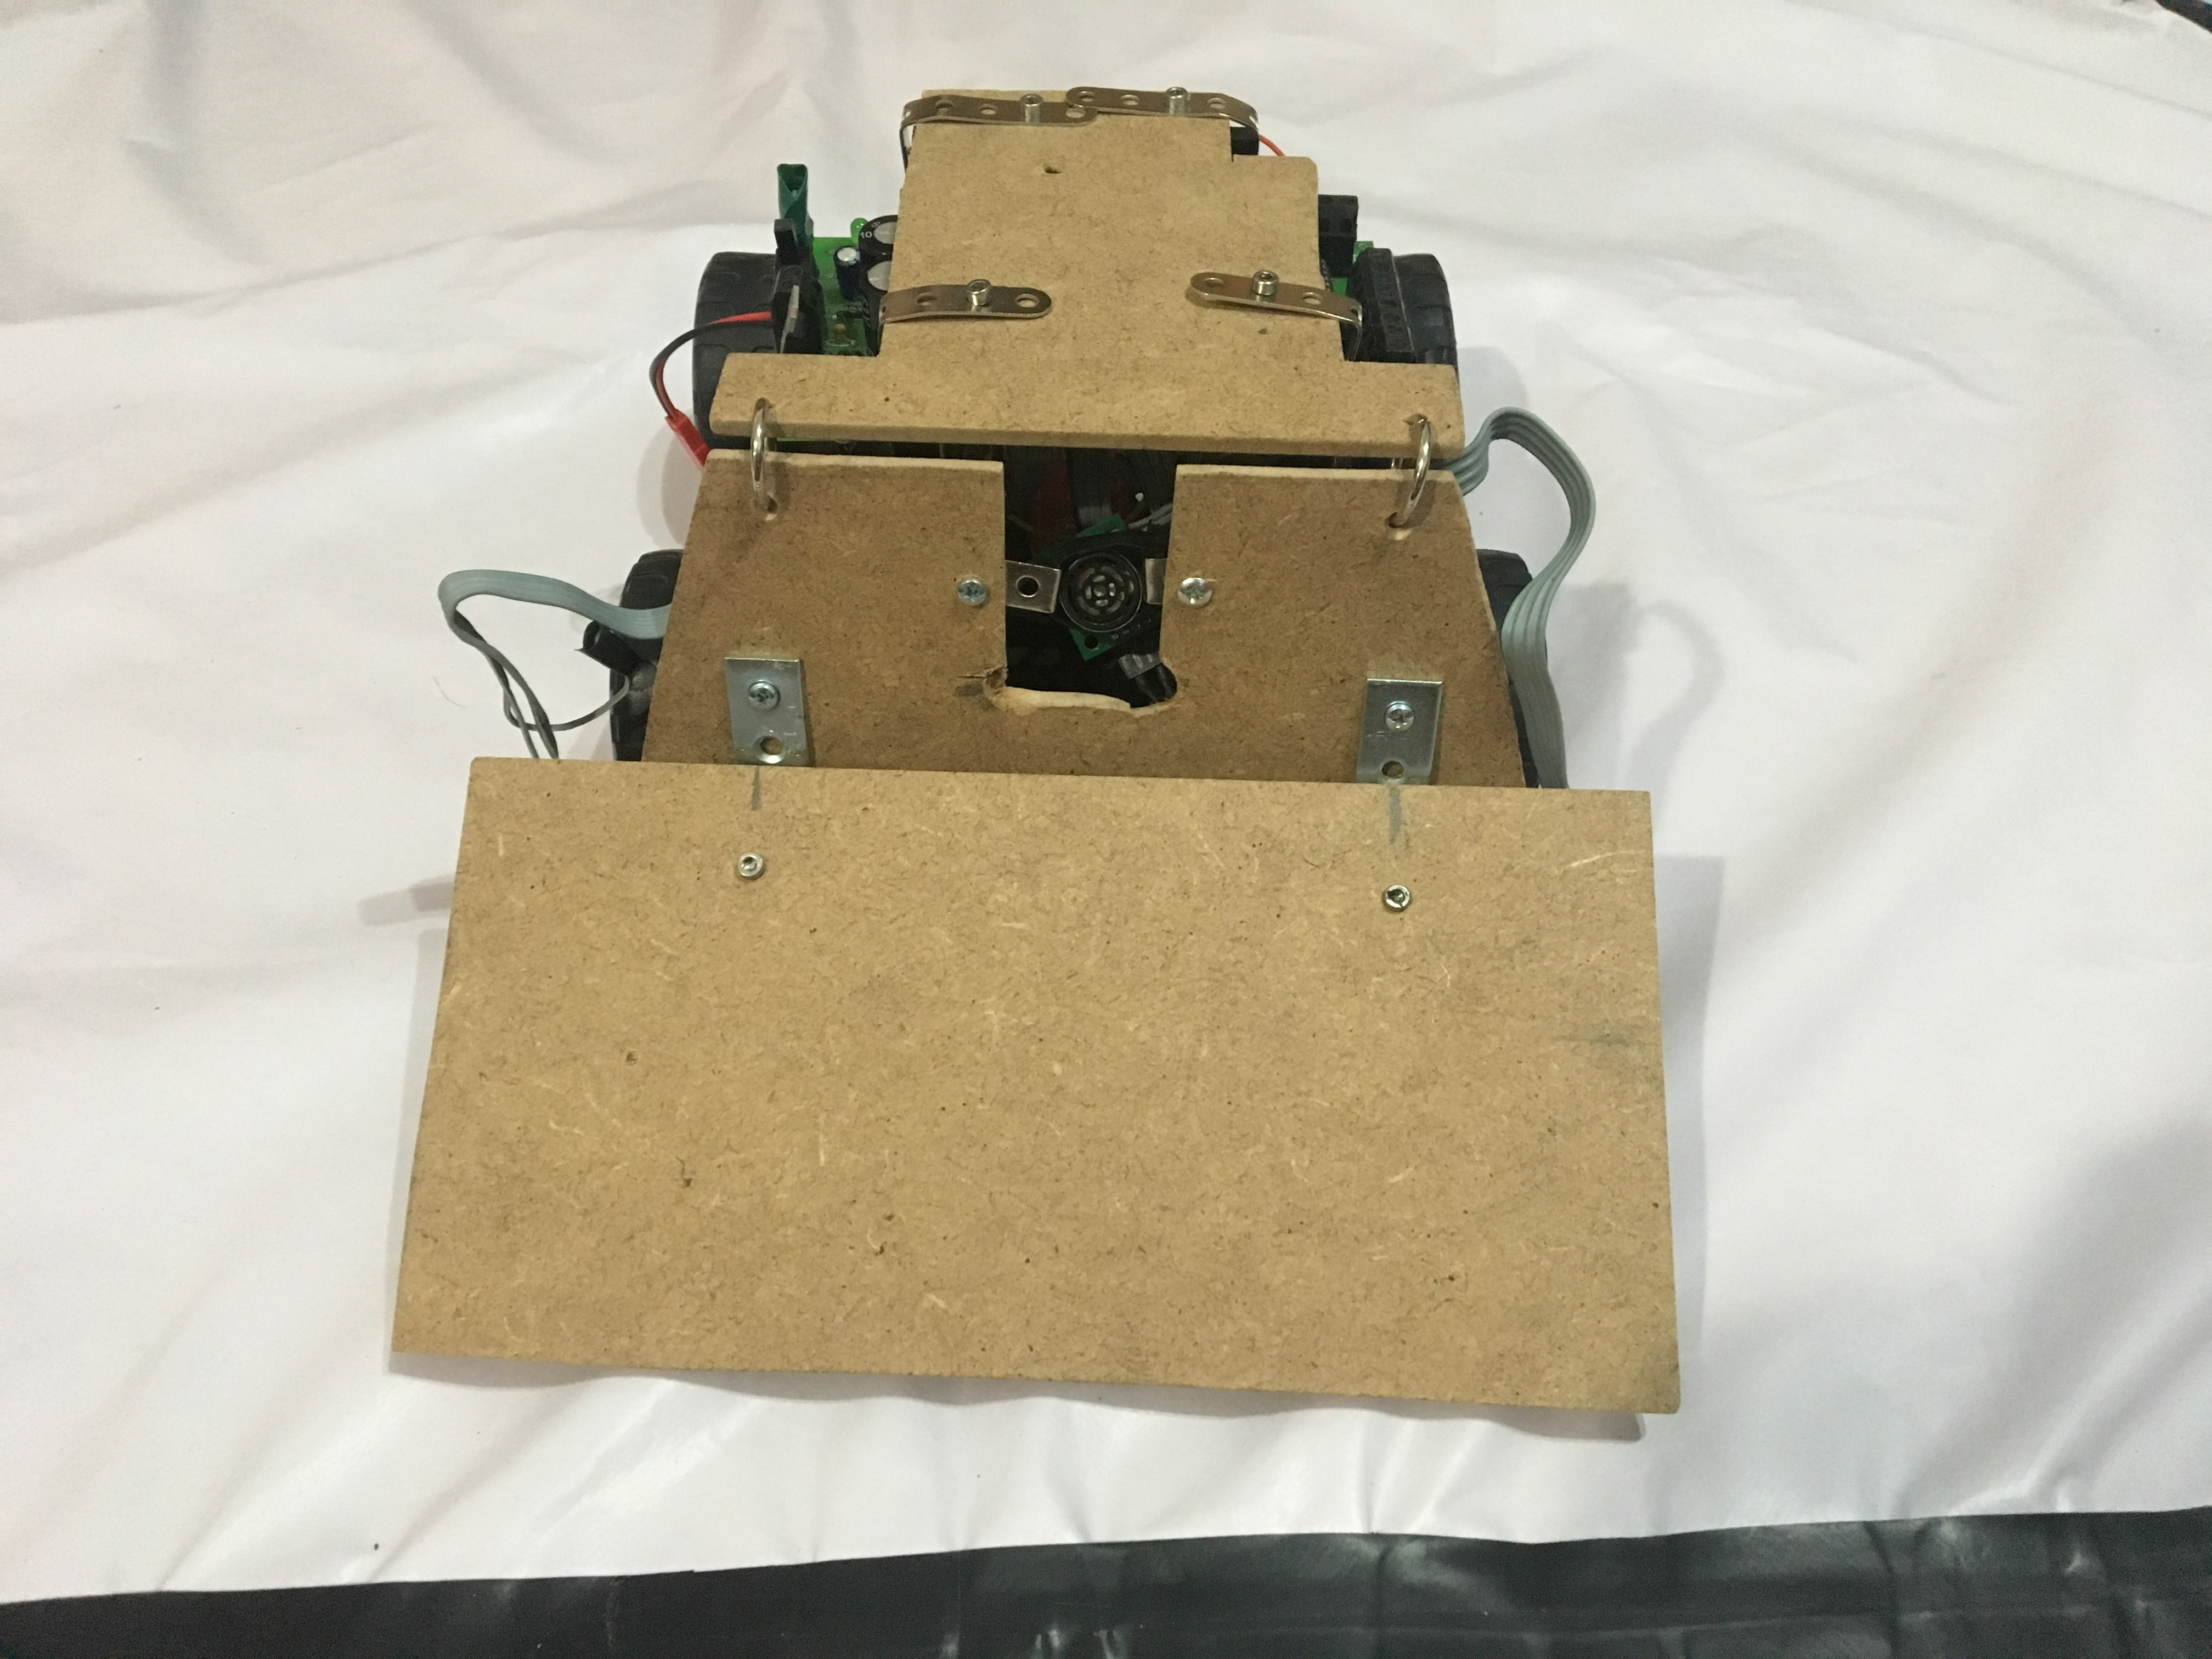
\includegraphics[scale=0.07]{./img/zigurat1}
    \end{figure}
\end{frame}

\begin{frame}{Hardware empleado (3)}
  \begin{figure}
    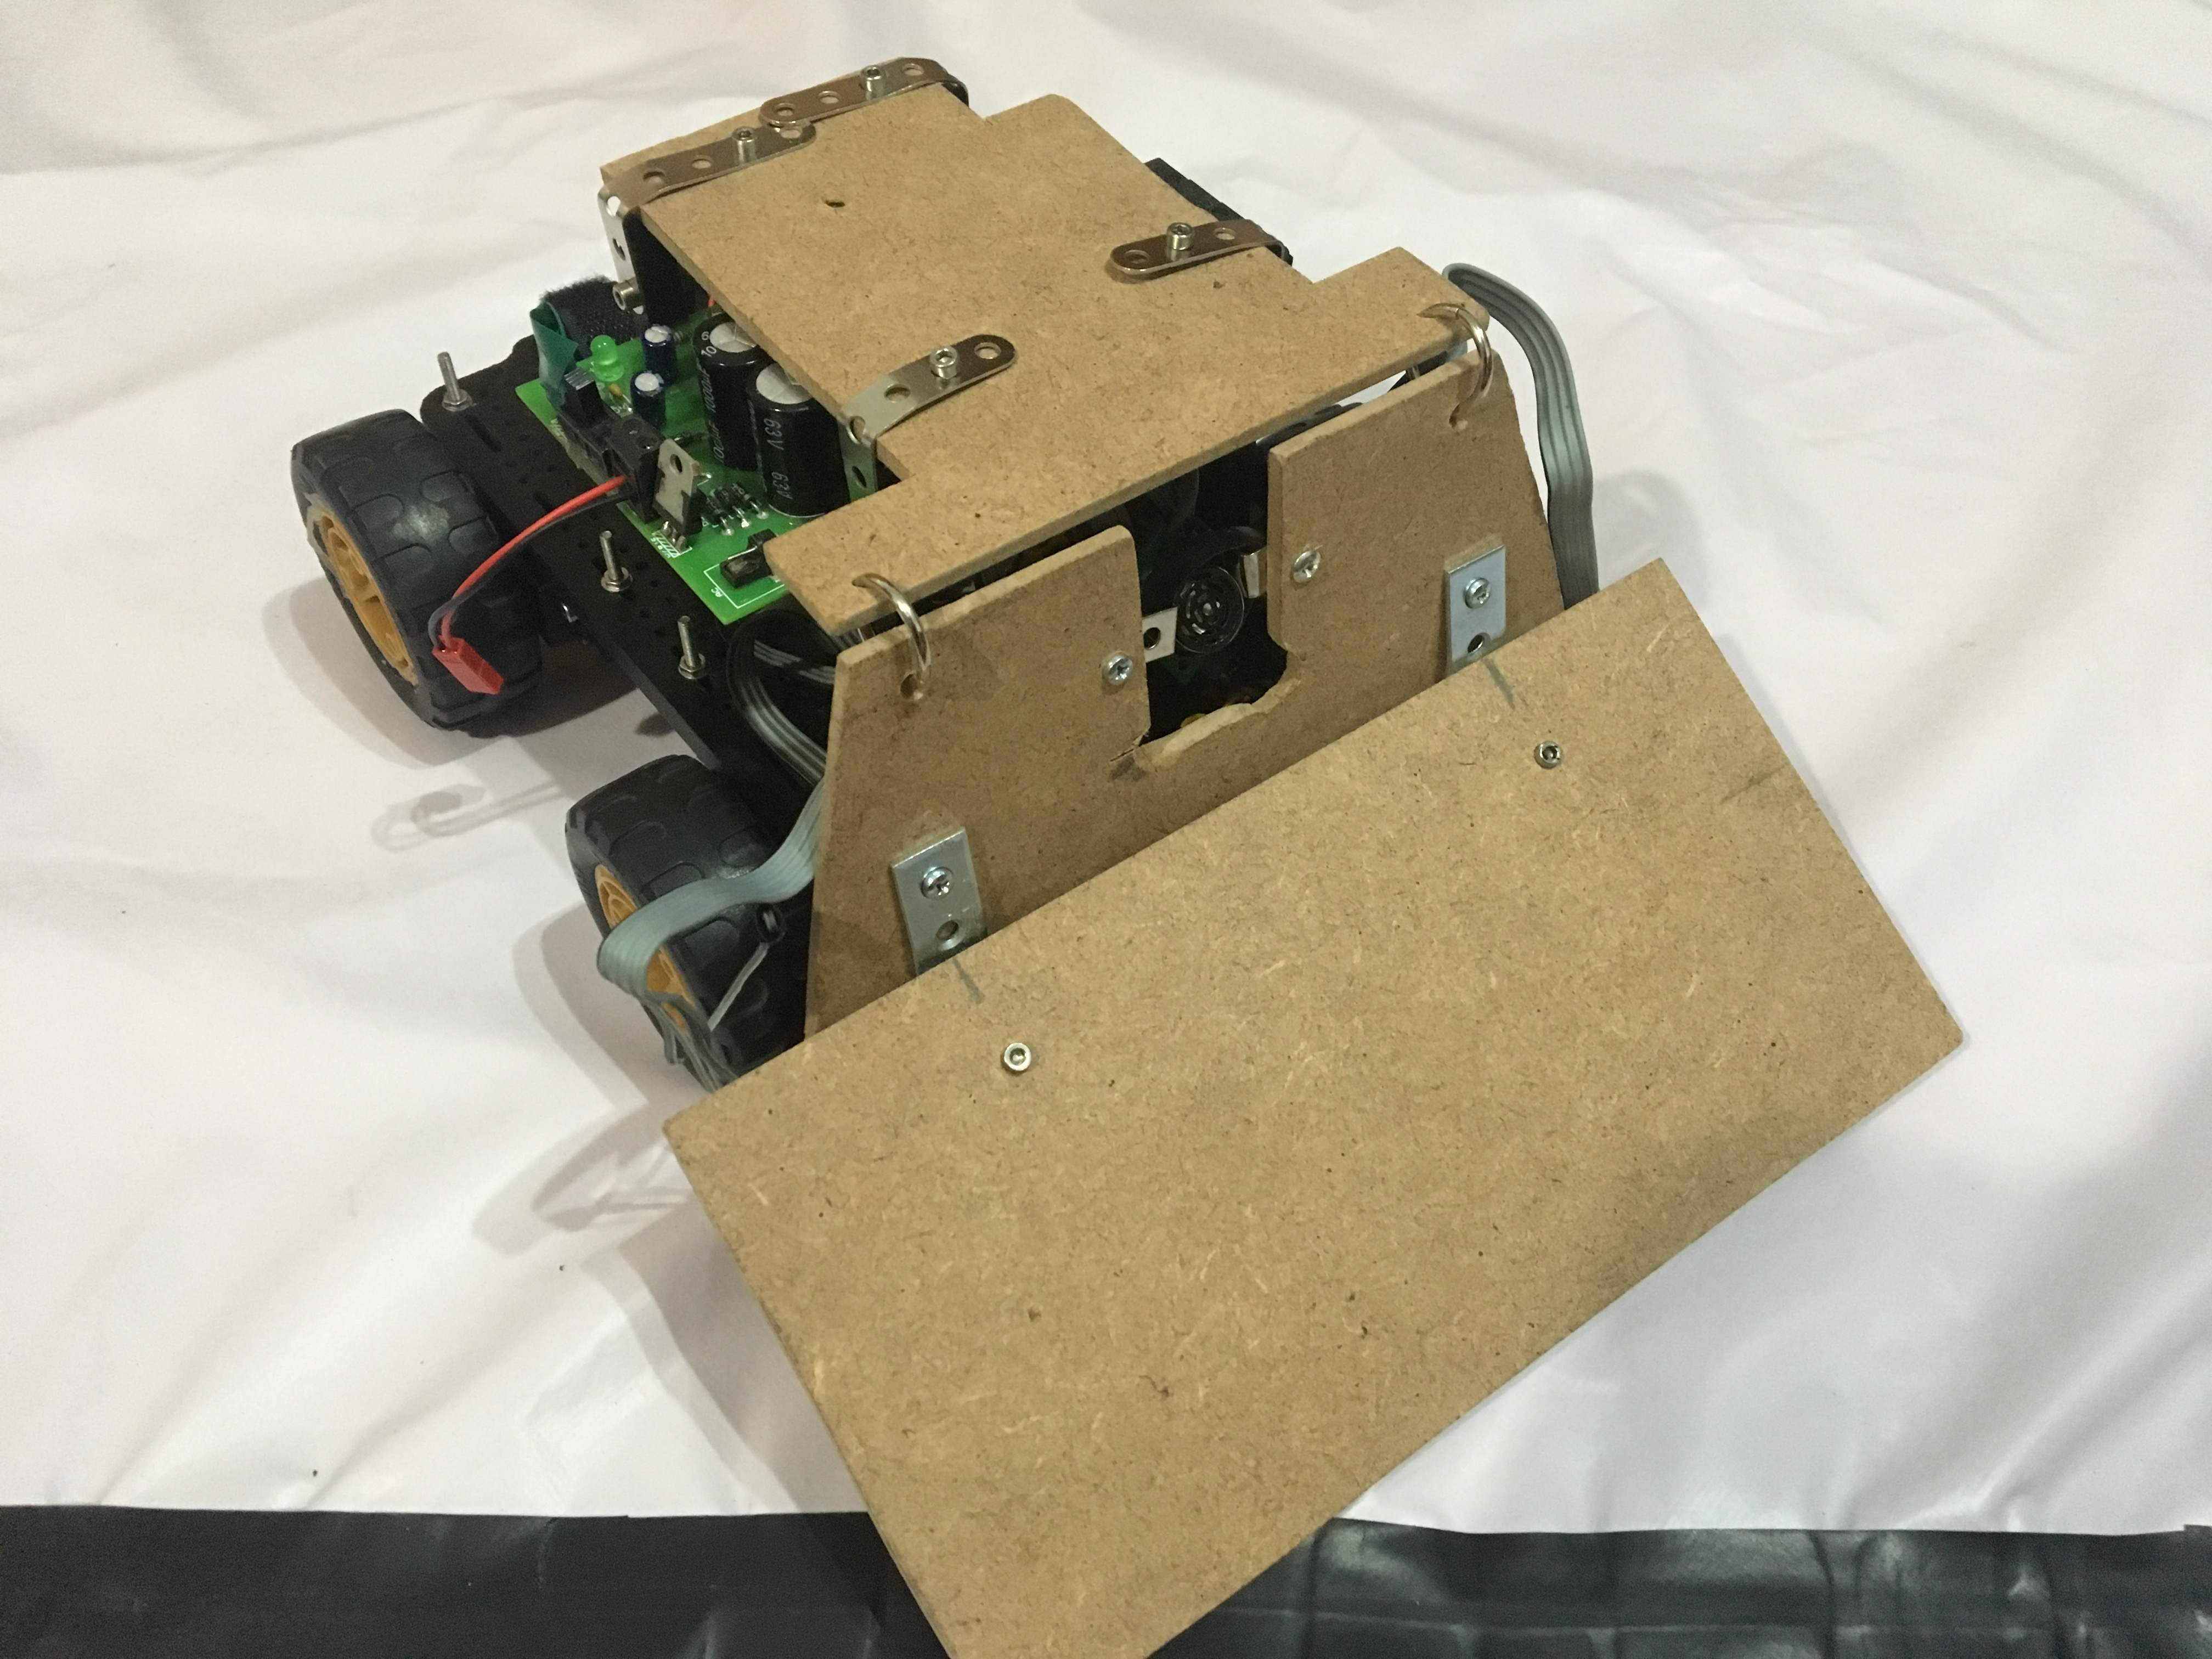
\includegraphics[scale=0.07]{./img/zigurat2}
    \end{figure}
\end{frame}

\begin{frame}{Hardware empleado (4)}
  \begin{figure}
    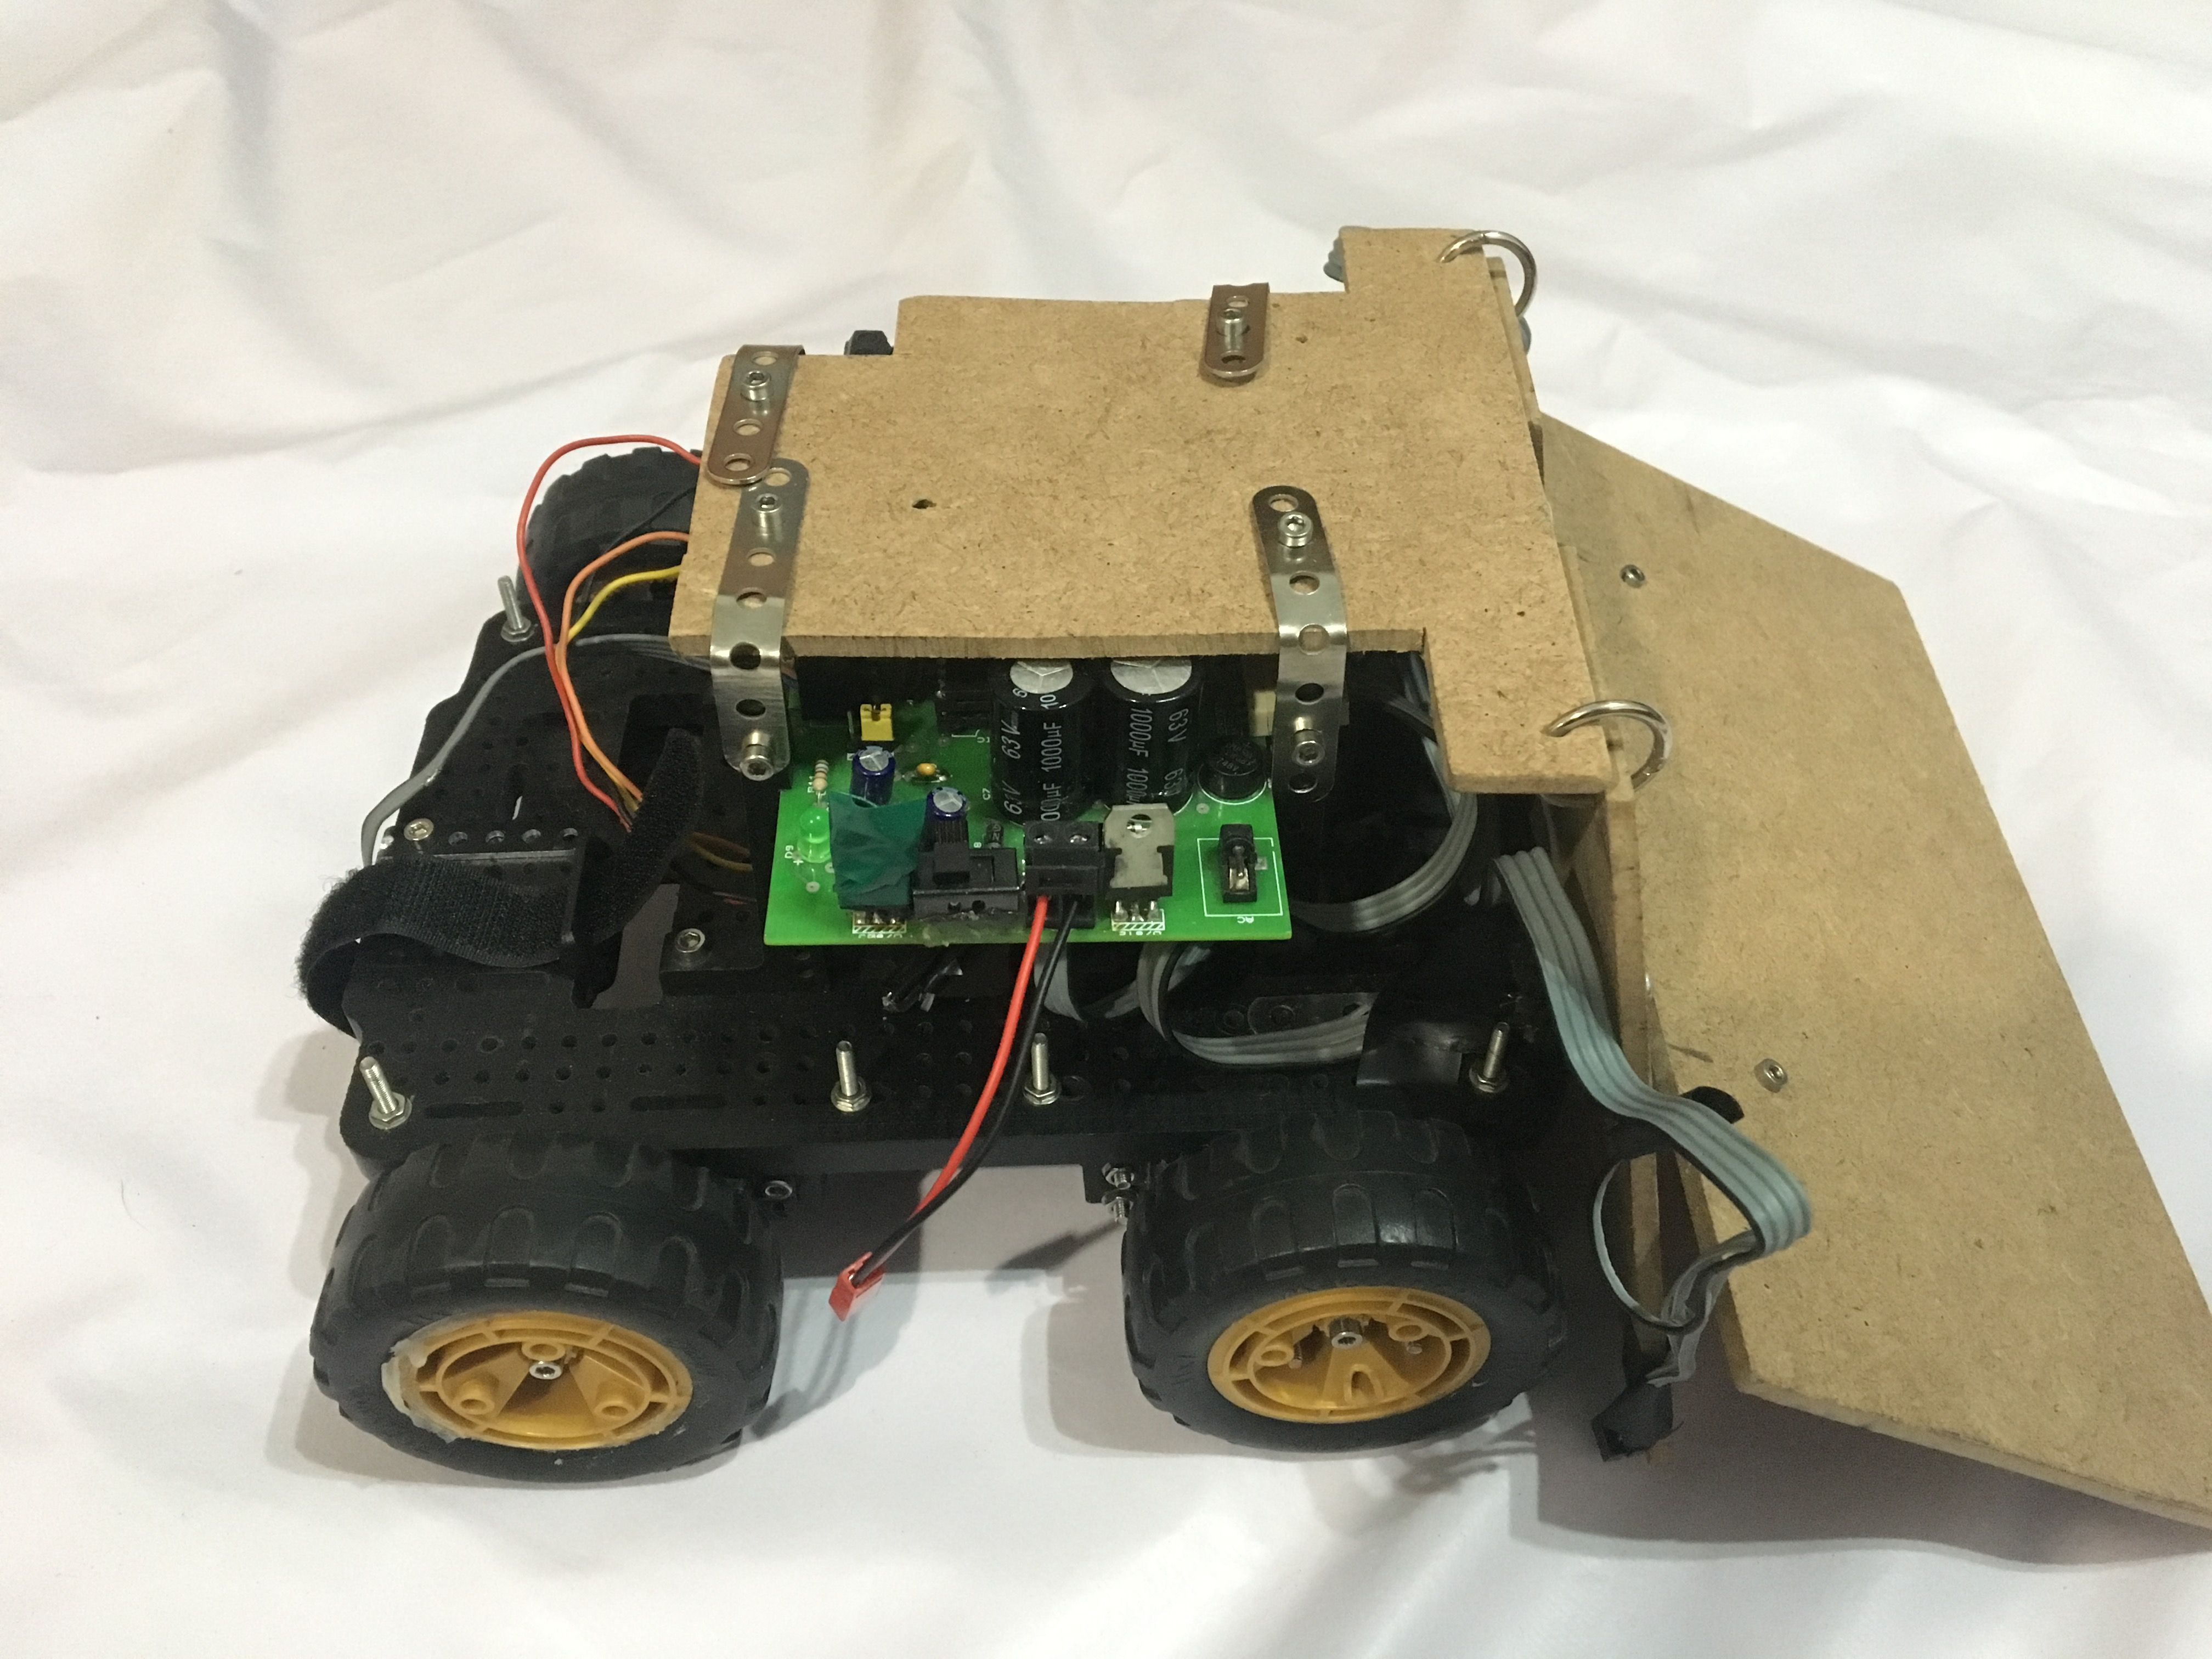
\includegraphics[scale=0.07]{./img/zigurat3}
    \end{figure}
\end{frame}

\begin{frame}{Hardware empleado (5)}
  \begin{figure}
    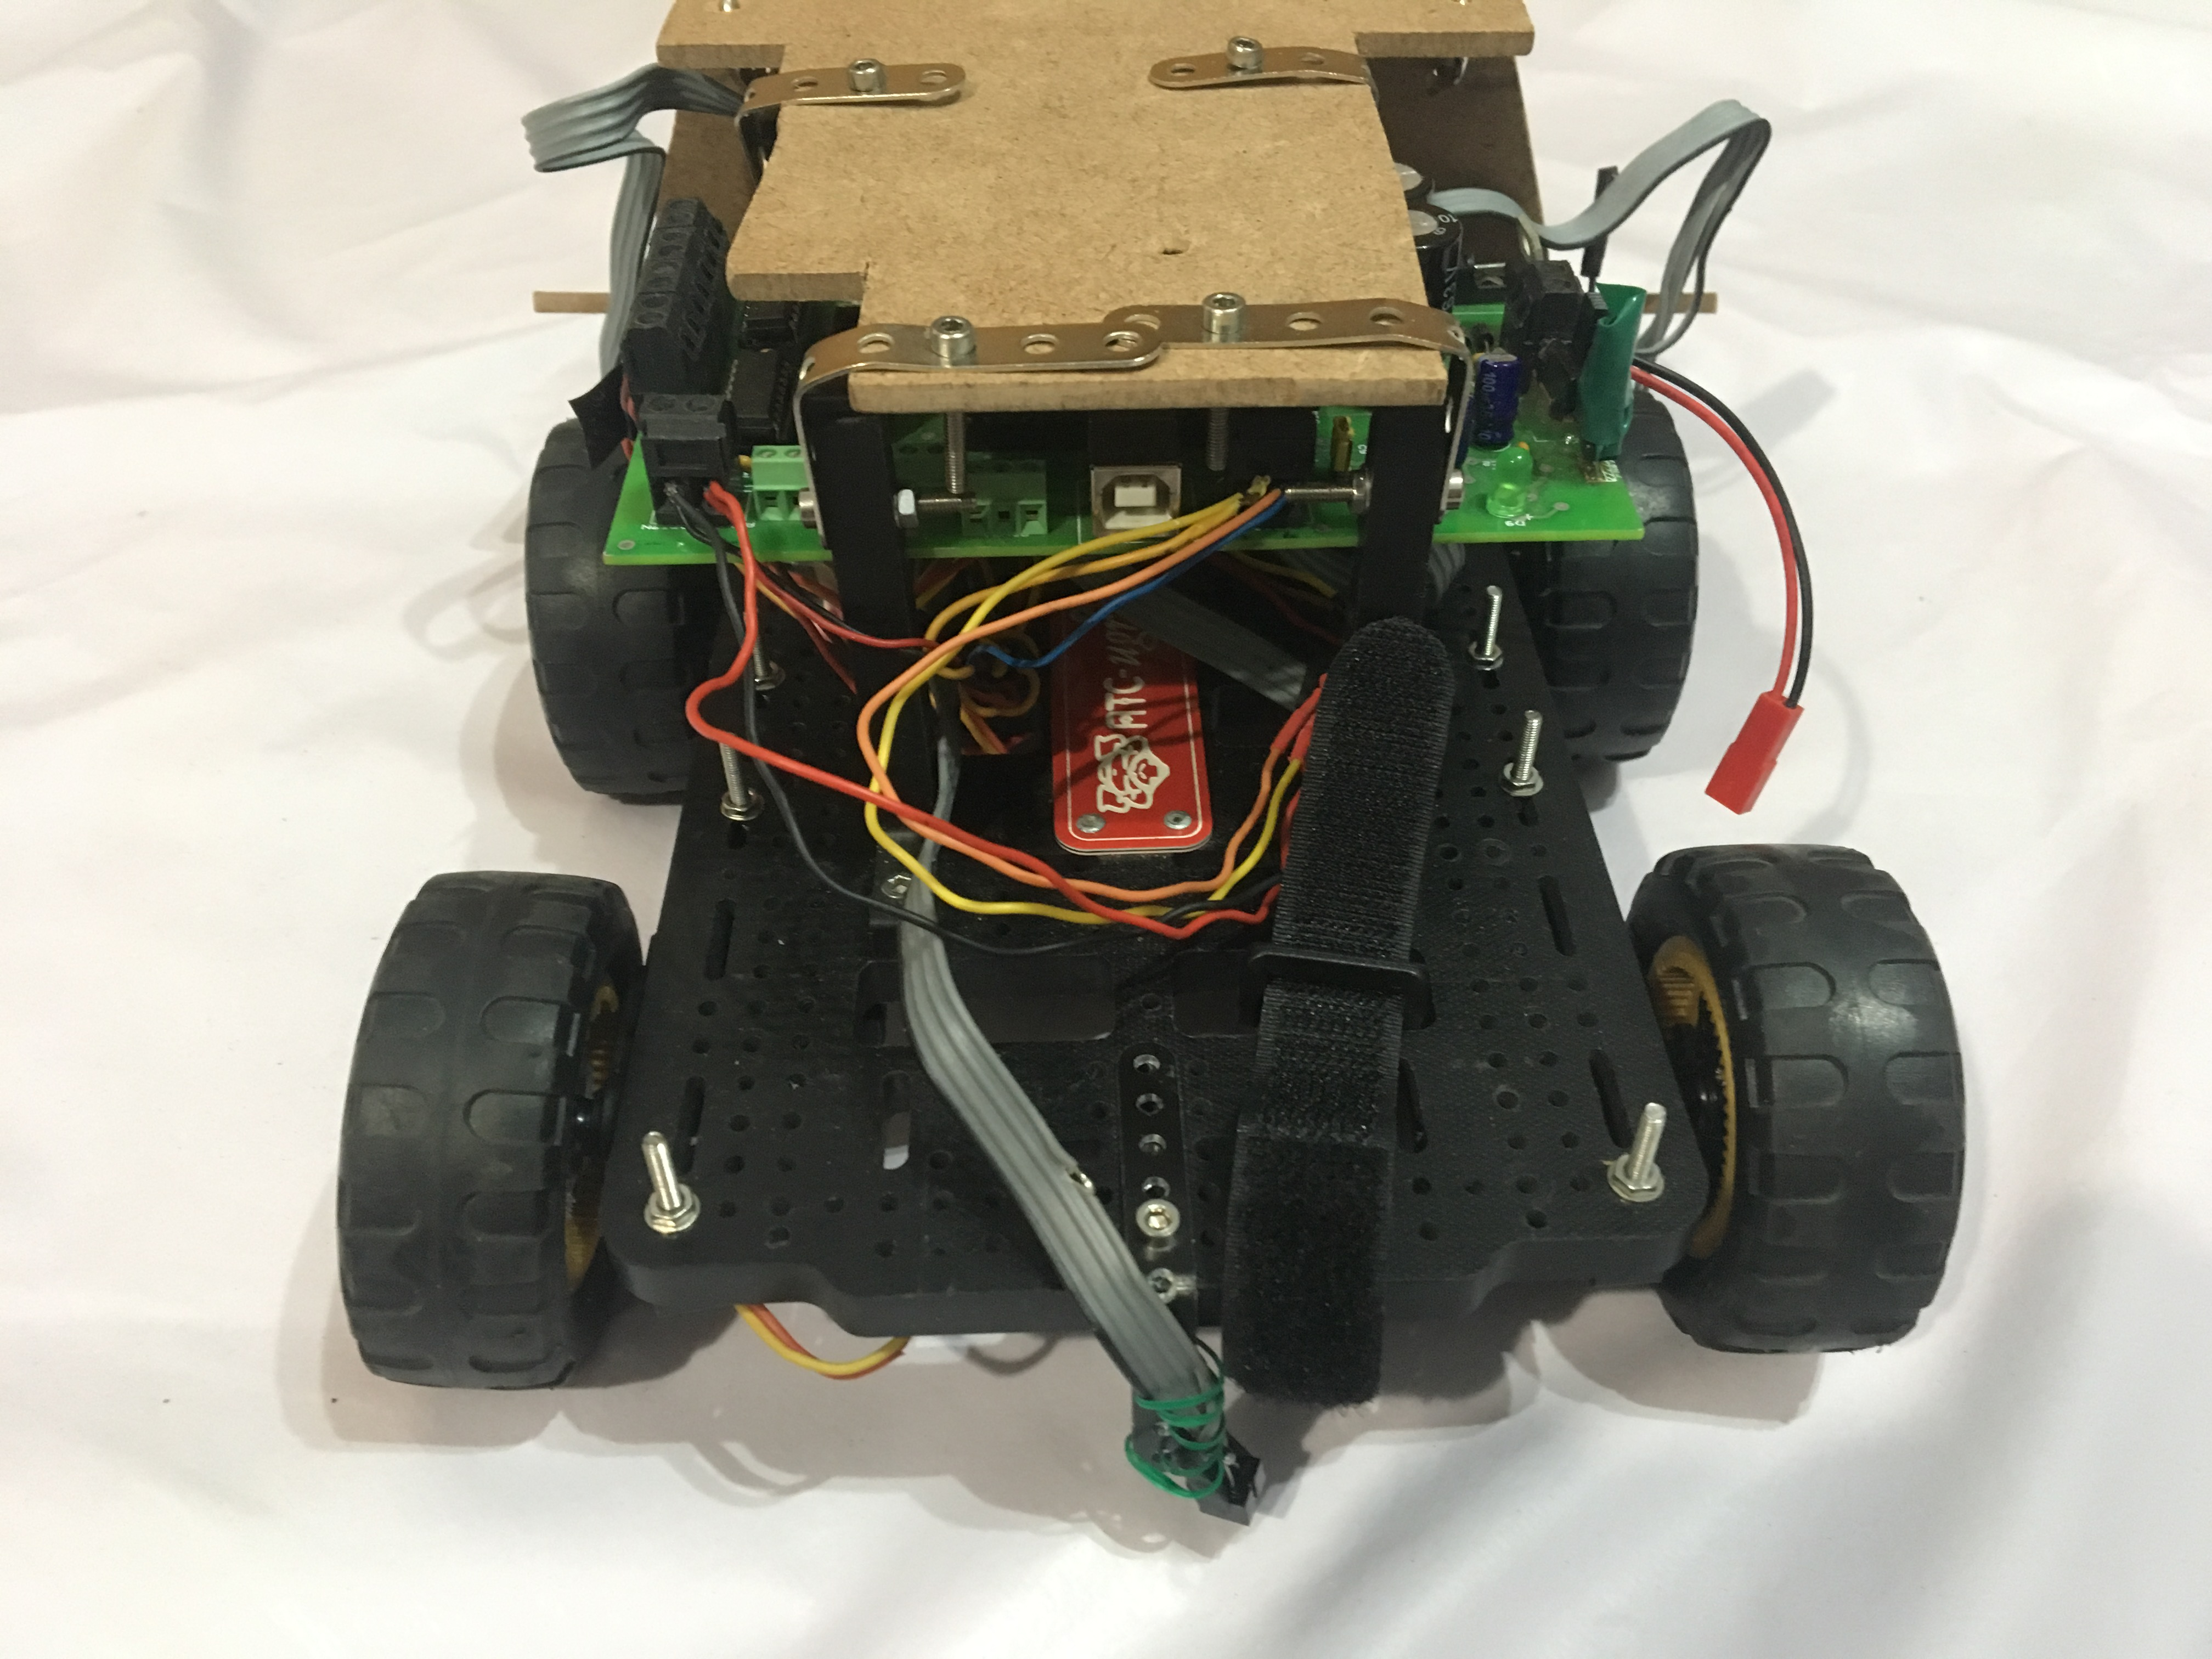
\includegraphics[scale=0.07]{./img/zigurat4}
    \end{figure}
\end{frame}

\begin{frame}{Un Zigurat}
  \begin{figure}
    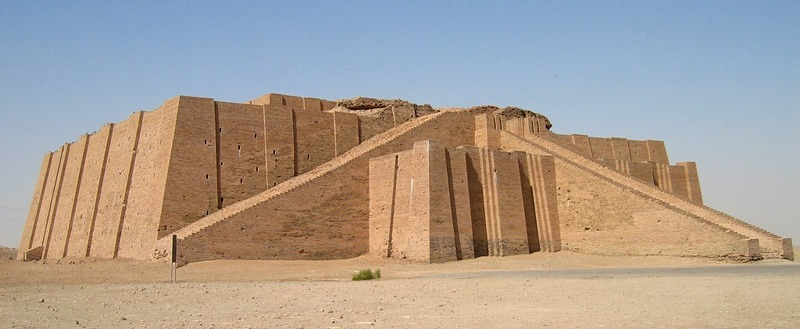
\includegraphics[scale=0.5]{./img/zigurat-mesopotamico}
    \end{figure}
\end{frame}

\begin{frame}{Programa}
  \begin{itemize}
    \item El programa del robot funciona mediante estados.
    \item Al principio el robot se encuentra en estado inicial y pasa al estado explorar. En función de la información que recibe de los distintos sensores, cambia de estado.
    \item El orden de prioridad de los sensores es (de mayor a menor prioridad): bumpers, sensor de línea negra trasero, sensores de línea negra delanteros. 
  \end{itemize}
\end{frame}

\begin{frame}{Estados (1)}
  \begin{itemize}
    \item EXPLORAR. El robot gira sobre su propio eje hacia la derecha a velocidad reducida. Si encuentra un objeto a una distancia entre 30 y 100 centímetros, se acerca a él. En cuanto está a menos de 30 centímetros, pasa al estado LAPA.
    \item LAPA. El robot comprueba el estado de los bumpers e intenta ponerse frente al otro robot. Cuando está de frente, empuja hacia delante a máxima velocidad.
  \end{itemize}
\end{frame}

\begin{frame}{Estados (2)}
  \begin{itemize}
    \item HUIR. El robot ha detectado la línea negra por detrás. Procede a girar sobre su propio eje e intentar avanzar hacia delante para no salirse.
    \item EVITAR\_LD. El robot ha detectado la línea negra por delante (a derecha o izquierda) y gira para evitarla.
  \end{itemize}
\end{frame}

\begin{frame}[fragile]{Diagrama de estados}
  \begin{tikzpicture}[node distance=4cm]
    \small 
    \node[state, initial] (q1) {INICIAL};
    \node[state, right of=q1] (q2) {EXPLORAR};
    \node[state, right of=q2] (q3) {HUIR};
    \node[state, below of=q1] (q4) {EVITAR\_LD};
    \node[state, right of=q4] (q5) {LAPA};
    \path[->]
    (q1) edge [above] node{} (q2)
    (q2) edge [sloped, bend left, align=center, below] node{Bumper} (q5)
    (q5) edge [sloped, align=center] node{} (q2)
    (q2) edge [sloped, anchor=center, bend right, below] node{SRF02} (q5)
    (q5) edge [sloped, bend right, below] node{CNY Trasero} (q3)
    (q2) edge [sloped, below] node{CNY Delantero} (q4)
    (q4) edge [bend left, sloped, above] node{} (q2)
    (q2) edge [bend left, above] node{CNY Trasero} (q3)
    (q3) edge [bend left, below] node{} (q2)
    (q2) edge [loop above] node{} (q2);
  \end{tikzpicture}
\end{frame}

\end{document}

